\documentclass[]{article}
\usepackage{lmodern}
\usepackage{amssymb,amsmath}
\usepackage{ifxetex,ifluatex}
\usepackage{fixltx2e} % provides \textsubscript
\ifnum 0\ifxetex 1\fi\ifluatex 1\fi=0 % if pdftex
  \usepackage[T1]{fontenc}
  \usepackage[utf8]{inputenc}
\else % if luatex or xelatex
  \ifxetex
    \usepackage{mathspec}
    \usepackage{xltxtra,xunicode}
  \else
    \usepackage{fontspec}
  \fi
  \defaultfontfeatures{Mapping=tex-text,Scale=MatchLowercase}
  \newcommand{\euro}{€}
\fi
% use upquote if available, for straight quotes in verbatim environments
\IfFileExists{upquote.sty}{\usepackage{upquote}}{}
% use microtype if available
\IfFileExists{microtype.sty}{%
\usepackage{microtype}
\UseMicrotypeSet[protrusion]{basicmath} % disable protrusion for tt fonts
}{}
\ifxetex
  \usepackage[setpagesize=false, % page size defined by xetex
              unicode=false, % unicode breaks when used with xetex
              xetex]{hyperref}
\else
  \usepackage[unicode=true]{hyperref}
\fi
\hypersetup{breaklinks=true,
            bookmarks=true,
            pdfauthor={},
            pdftitle={},
            colorlinks=true,
            citecolor=blue,
            urlcolor=blue,
            linkcolor=magenta,
            pdfborder={0 0 0}}
\urlstyle{same}  % don't use monospace font for urls
\usepackage{color}
\usepackage{fancyvrb}
\newcommand{\VerbBar}{|}
\newcommand{\VERB}{\Verb[commandchars=\\\{\}]}
\DefineVerbatimEnvironment{Highlighting}{Verbatim}{commandchars=\\\{\}}
% Add ',fontsize=\small' for more characters per line
\newenvironment{Shaded}{}{}
\newcommand{\KeywordTok}[1]{\textcolor[rgb]{0.00,0.44,0.13}{\textbf{{#1}}}}
\newcommand{\DataTypeTok}[1]{\textcolor[rgb]{0.56,0.13,0.00}{{#1}}}
\newcommand{\DecValTok}[1]{\textcolor[rgb]{0.25,0.63,0.44}{{#1}}}
\newcommand{\BaseNTok}[1]{\textcolor[rgb]{0.25,0.63,0.44}{{#1}}}
\newcommand{\FloatTok}[1]{\textcolor[rgb]{0.25,0.63,0.44}{{#1}}}
\newcommand{\ConstantTok}[1]{\textcolor[rgb]{0.53,0.00,0.00}{{#1}}}
\newcommand{\CharTok}[1]{\textcolor[rgb]{0.25,0.44,0.63}{{#1}}}
\newcommand{\SpecialCharTok}[1]{\textcolor[rgb]{0.25,0.44,0.63}{{#1}}}
\newcommand{\StringTok}[1]{\textcolor[rgb]{0.25,0.44,0.63}{{#1}}}
\newcommand{\VerbatimStringTok}[1]{\textcolor[rgb]{0.25,0.44,0.63}{{#1}}}
\newcommand{\SpecialStringTok}[1]{\textcolor[rgb]{0.73,0.40,0.53}{{#1}}}
\newcommand{\ImportTok}[1]{{#1}}
\newcommand{\CommentTok}[1]{\textcolor[rgb]{0.38,0.63,0.69}{\textit{{#1}}}}
\newcommand{\DocumentationTok}[1]{\textcolor[rgb]{0.73,0.13,0.13}{\textit{{#1}}}}
\newcommand{\AnnotationTok}[1]{\textcolor[rgb]{0.38,0.63,0.69}{\textbf{\textit{{#1}}}}}
\newcommand{\CommentVarTok}[1]{\textcolor[rgb]{0.38,0.63,0.69}{\textbf{\textit{{#1}}}}}
\newcommand{\OtherTok}[1]{\textcolor[rgb]{0.00,0.44,0.13}{{#1}}}
\newcommand{\FunctionTok}[1]{\textcolor[rgb]{0.02,0.16,0.49}{{#1}}}
\newcommand{\VariableTok}[1]{\textcolor[rgb]{0.10,0.09,0.49}{{#1}}}
\newcommand{\ControlFlowTok}[1]{\textcolor[rgb]{0.00,0.44,0.13}{\textbf{{#1}}}}
\newcommand{\OperatorTok}[1]{\textcolor[rgb]{0.40,0.40,0.40}{{#1}}}
\newcommand{\BuiltInTok}[1]{{#1}}
\newcommand{\ExtensionTok}[1]{{#1}}
\newcommand{\PreprocessorTok}[1]{\textcolor[rgb]{0.74,0.48,0.00}{{#1}}}
\newcommand{\AttributeTok}[1]{\textcolor[rgb]{0.49,0.56,0.16}{{#1}}}
\newcommand{\RegionMarkerTok}[1]{{#1}}
\newcommand{\InformationTok}[1]{\textcolor[rgb]{0.38,0.63,0.69}{\textbf{\textit{{#1}}}}}
\newcommand{\WarningTok}[1]{\textcolor[rgb]{0.38,0.63,0.69}{\textbf{\textit{{#1}}}}}
\newcommand{\AlertTok}[1]{\textcolor[rgb]{1.00,0.00,0.00}{\textbf{{#1}}}}
\newcommand{\ErrorTok}[1]{\textcolor[rgb]{1.00,0.00,0.00}{\textbf{{#1}}}}
\newcommand{\NormalTok}[1]{{#1}}
\usepackage{longtable,booktabs}
\usepackage{graphicx,grffile}
\makeatletter
\def\maxwidth{\ifdim\Gin@nat@width>\linewidth\linewidth\else\Gin@nat@width\fi}
\def\maxheight{\ifdim\Gin@nat@height>\textheight\textheight\else\Gin@nat@height\fi}
\makeatother
% Scale images if necessary, so that they will not overflow the page
% margins by default, and it is still possible to overwrite the defaults
% using explicit options in \includegraphics[width, height, ...]{}
\setkeys{Gin}{width=\maxwidth,height=\maxheight,keepaspectratio}
\setlength{\parindent}{0pt}
\setlength{\parskip}{6pt plus 2pt minus 1pt}
\setlength{\emergencystretch}{3em}  % prevent overfull lines
\providecommand{\tightlist}{%
  \setlength{\itemsep}{0pt}\setlength{\parskip}{0pt}}
\setcounter{secnumdepth}{0}

\date{}

% Redefines (sub)paragraphs to behave more like sections
\ifx\paragraph\undefined\else
\let\oldparagraph\paragraph
\renewcommand{\paragraph}[1]{\oldparagraph{#1}\mbox{}}
\fi
\ifx\subparagraph\undefined\else
\let\oldsubparagraph\subparagraph
\renewcommand{\subparagraph}[1]{\oldsubparagraph{#1}\mbox{}}
\fi

\begin{document}
	\title{\huge\textbf{ArUco Markers}\LARGE \\Project: Marker-based Localization}
	\author{Niharika Jayanthi, Dheeraj Kamath \\Mentor: Sanam Shakya}
	\maketitle
	\pagebreak
\section{Goal}\label{goal}

In this documentation, we shall learn-

\begin{itemize}
\tightlist
\item
  ArUco markers; encoding and decoding
\item
  How to detect and decode markers from video feed
\end{itemize}

\section{Prerequisites}\label{prerequisites}

\begin{itemize}
\tightlist
\item
  Hamming code
\end{itemize}

\section{Theory}\label{theory}

\subsection{Introduction}\label{introduction}

ArUco marker is a 5x5 grid that is black and white in color. ArUco
markers are based on Hamming code. In the grid, the first, third and
fifth columns represent parity bits. The second and fourth columns
represent the data bits. Hence, there are ten total data bits. So the
maximum number of markers that can be encoded are-

2\^{}10 = 1024

\emph{\textbf{Encoding}}

Let us consider the number 650. It's binary representation is
1010001010. There are two data bits in each row.

\begin{figure}[htbp]
\centering
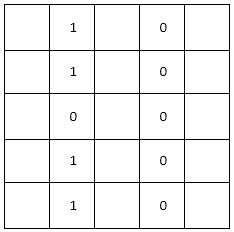
\includegraphics{images/Aruco markers/1.JPG}
\caption{Data rows}
\end{figure}

Now, each row is encoded separately using slightly modified Hamming
code. The first and third parity bits are calculated using even parity
while the second parity bit uses odd parity. We get the following
encoded values-

\begin{longtable}[c]{@{}lllll@{}}
\toprule
Data bit 2 & Parity bit 3 & Data bit 1 & Parity bit 2 & Parity bit
1\tabularnewline
\midrule
\endhead
0 & 0 & 1 & 0 & 1\tabularnewline
0 & 0 & 1 & 0 & 1\tabularnewline
0 & 0 & 0 & 1 & 0\tabularnewline
0 & 0 & 1 & 0 & 1\tabularnewline
0 & 0 & 1 & 0 & 1\tabularnewline
\bottomrule
\end{longtable}

We rearrange the bits in each row and get the following result-

\begin{figure}[htbp]
\centering
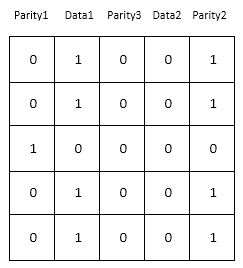
\includegraphics{images/Aruco markers/2.JPG}
\caption{ArUco bits for 0b1010001010}
\end{figure}

If the cell value is 0, color it black; if value is 1, color it white.
This will give us the ArUco marker-

\begin{figure}[htbp]
\centering

\includegraphics[width = 8cm]{images/Aruco markers/3.png}
\caption{ArUco marker}
\end{figure}

The above marker is padded with one layer of black cells.

\emph{\textbf{Decoding}}

After understanding the above section, decoding is an extremely simple
process. The following steps are to be followed while decoding a
perfect, computer-generated image of an ArUco marker.

\textbf{Step 1} : Extract the ArUco from the image.

\textbf{Step 2} : Remove the extra padding.

\textbf{Step 3} : Divide the resulting image into a 5x5 grid and check
the color in each cell of the second and fourth columns(in that order)
in a top to bottom manner.

\textbf{Step 4} : If the color is white, write 1; else, write it 0.

\textbf{Step 5} : The resulting number will be in binary. Convert it
into decimal

\subsection{Applications}\label{applications}

\begin{itemize}
\tightlist
\item
  These markers are utilized in augmented reality applications.
\item
  They can be used in robot navigation algorithms.
\end{itemize}

\section{Code}\label{code}

The main functions used are -

\href{https://github.com/eyantrainternship/eYSIP_2015_Marker_based_Robot_Localisation/wiki/Thresholding}{cv2.threshold()}

\href{https://github.com/eyantrainternship/eYSIP_2015_Marker_based_Robot_Localisation/wiki/Contour-Features-and-Shape-Detection}{cv2.approxPolyDP()}

The code is written using the above-mentioned steps:

\begin{Shaded}
\begin{Highlighting}[]
\CommentTok{#Imports}

\ImportTok{import} \NormalTok{cv2}

\CommentTok{#Define globals}

\NormalTok{MAX_SIZE }\OperatorTok{=} \DecValTok{406}

\CommentTok{#Define helper functions}

\KeywordTok{def} \NormalTok{extractAruco(img):}
    
    \CommentTok{#Inverse threshold to get the inner contour}
    \NormalTok{gray }\OperatorTok{=} \NormalTok{cv2.cvtColor(img, cv2.COLOR_BGR2GRAY)}
    \NormalTok{ret, th }\OperatorTok{=} \NormalTok{cv2.threshold(gray, }\DecValTok{127}\NormalTok{,}\DecValTok{255}\NormalTok{,cv2.THRESH_BINARY_INV)}

    \CommentTok{#Crop image}
    \NormalTok{contours, hierarchy }\OperatorTok{=} \NormalTok{cv2.findContours(th, cv2.RETR_EXTERNAL,}
                                           \NormalTok{cv2.CHAIN_APPROX_SIMPLE)}
    \NormalTok{contours }\OperatorTok{=} \NormalTok{contours[}\DecValTok{0}\NormalTok{]}

    \NormalTok{epsilon }\OperatorTok{=} \FloatTok{0.1}\OperatorTok{*}\NormalTok{cv2.arcLength(contours,}\VariableTok{True}\NormalTok{)}
    \NormalTok{approx }\OperatorTok{=} \NormalTok{cv2.approxPolyDP(contours,epsilon,}\VariableTok{True}\NormalTok{)}

    \NormalTok{image_crop}\OperatorTok{=}\NormalTok{gray[approx[}\DecValTok{0}\NormalTok{,}\DecValTok{0}\NormalTok{,}\DecValTok{1}\NormalTok{]:approx[}\DecValTok{2}\NormalTok{,}\DecValTok{0}\NormalTok{,}\DecValTok{1}\NormalTok{],approx[}\DecValTok{0}\NormalTok{,}\DecValTok{0}\NormalTok{,}\DecValTok{0}\NormalTok{]:approx[}\DecValTok{2}\NormalTok{,}\DecValTok{0}\NormalTok{,}\DecValTok{0}\NormalTok{]]}

    \CommentTok{#Return extracted image}
    \ControlFlowTok{return} \NormalTok{image_crop}


\KeywordTok{def} \NormalTok{findArucoID(inp_img):}

    \CommentTok{#Extract image}
    \NormalTok{im }\OperatorTok{=} \NormalTok{extractAruco(inp_img)}

    \CommentTok{#Resize it to smaller size for check}
    \NormalTok{im }\OperatorTok{=} \NormalTok{cv2.resize(im, (MAX_SIZE,MAX_SIZE))}

    \CommentTok{#Remove padding}
    \NormalTok{width }\OperatorTok{=} \NormalTok{MAX_SIZE }\OperatorTok{/} \DecValTok{7}
    \NormalTok{im }\OperatorTok{=} \NormalTok{im[width:width}\OperatorTok{*}\DecValTok{6}\NormalTok{,width:width}\OperatorTok{*}\DecValTok{6}\NormalTok{]}

    \CommentTok{#Calculate ID}
    \NormalTok{ret_val }\OperatorTok{=} \DecValTok{0}
    
    \ControlFlowTok{for} \NormalTok{y }\OperatorTok{in} \BuiltInTok{range}\NormalTok{(}\DecValTok{5}\NormalTok{):}
        \NormalTok{_val1 }\OperatorTok{=} \BuiltInTok{int}\NormalTok{(im[(y }\OperatorTok{*} \NormalTok{width) }\OperatorTok{+}  \NormalTok{(width }\OperatorTok{/} \DecValTok{2}\NormalTok{), width }\OperatorTok{+} \NormalTok{width }\OperatorTok{/} \DecValTok{2}\NormalTok{]) }\CommentTok{#im[y, x] format}
        \NormalTok{_val2 }\OperatorTok{=} \BuiltInTok{int}\NormalTok{(im[(y }\OperatorTok{*} \NormalTok{width) }\OperatorTok{+}  \NormalTok{(width }\OperatorTok{/} \DecValTok{2}\NormalTok{), }\DecValTok{3} \OperatorTok{*} \NormalTok{width }\OperatorTok{+} \NormalTok{width }\OperatorTok{/} \DecValTok{2}\NormalTok{]) }\CommentTok{#im[y, x] format}

        \ControlFlowTok{if} \NormalTok{_val1 }\OperatorTok{==} \DecValTok{255}\NormalTok{:}
            \NormalTok{_val1 }\OperatorTok{=} \DecValTok{1}

        \ControlFlowTok{if} \NormalTok{_val2 }\OperatorTok{==} \DecValTok{255}\NormalTok{:}
            \NormalTok{_val2 }\OperatorTok{=} \DecValTok{1}

        
        \NormalTok{ret_val }\OperatorTok{=} \NormalTok{ret_val }\OperatorTok{*} \DecValTok{2} \OperatorTok{+} \NormalTok{_val1}
        \NormalTok{ret_val }\OperatorTok{=} \NormalTok{ret_val }\OperatorTok{*} \DecValTok{2} \OperatorTok{+} \NormalTok{_val2}

    \ControlFlowTok{return} \NormalTok{ret_val}
        


\NormalTok{image }\OperatorTok{=} \NormalTok{cv2.imread(}\StringTok{"your_example.png"}\NormalTok{)}
\NormalTok{ID }\OperatorTok{=} \NormalTok{findArucoID(image)}

\BuiltInTok{print} \StringTok{"Marker ID is"}\NormalTok{, ID}
\end{Highlighting}
\end{Shaded}

\section{Resources}\label{resources}

\begin{itemize}
\tightlist
\item
  http://www.uco.es/investiga/grupos/ava/node/26
\item
  http://iplimage.com/blog/create-markers-aruco/
\item
  http://terpconnect.umd.edu/\textasciitilde{}jwelsh12/enes100/markergen.html
\end{itemize}

\section{Exercises}\label{exercises}

\begin{itemize}
\tightlist
\item
  Write a code to decode markers present in an image taken by a camera.
\item
  How will you detect a rotated marker?
\end{itemize}

\end{document}
